\chapter{Related Studies}
\label{chp:pre_study}

\noindent In order to bridge the \gls{ip} network and telephony network, a solution to create a real-time communication channel between \gls{ip} network and \gls{voip} network is the key factor since the \gls{voip} network is the bridge to make \gls{ip} network to talk with telephony network. In this Chapter, some introduction of \gls{webrtc} and \gls{sip} network will be covered. \gls{sip} is one of the \gls{voip} signaling protocols widely used in current internet telephony service which is also the target telephony network in this thesis. There will be some studies of \gls{webrtc} business cases and prototype working scenario based on these \gls{webrtc} usage cases in this chapter. The prototype working scenario is designed by considering these different \gls{webrtc} usage cases.

\section{WebRTC}

\noindent Before \gls{webrtc} announced, Gmail\footnote{Gmail is a free , advertising-supported email service provided by Google.} video chat became popular in 2008, and in 2011 Google introduced Hangouts\footnote{Google Hangouts is an instant messaging and video chat platform developed by Google, which launched on May 15, 2013 during the keynote of its I/O development conference. It replaces three messaging products that Google had implemented concurrently within its services, including Talk, Google+ Messenger, and Hangouts, a video chat system present within Google+.}, which uses the Google Talk service (as does Gmail). In May 2011, Google released an open source project for browser-based real-time communication known as \gls{webrtc}. This has been followed by ongoing work to standardize the relevant protocols in the \gls{ietf} and browser \gls{api}s in the \gls{w3c}.

\subsection{What is WebRTC ?}

\noindent \gls{webrtc} is an industry and standards effort to put real-time communications capabilities into all browsers and make these capabilities accessible to web developers via standard \gls{html5} tags and JavaScript \gls{api}s. For example, consider functionality similar to that offered by Skype\footnote{Skype is a freemium voice-over-IP service and instant messaging client, currently developed by the Microsoft Skype Division.\cite{wiki:skype}}. but without installing any software or plug-ins. For a website or web application to work regardless of which browser is used, standards are required. Also, standards are required so that browsers can communicate with non-browsers, including enterprise and service provider telephony and communications equipment\cite{inbook:rtc-intro}.

\par With the rapidly development of internet, more and more communication traffic is moving to web from the traditional telephony network. And in the recent decade, \gls{voip} network services are growing to the peek of the market capacity. Solution to integrate \gls{webrtc} and existing \gls{voip} network is the right approach the trend of the internet communication requirement.

\subsection{WebRTC Network Structure}

\noindent In the Figure\ref{fig:webrtc_network_finCandidate}\cite{html5rock:webrtc} shows how the \gls{ice} framework\footnote{ICE is a framework for connecting peers, such as two video chat clients.\cite{wiki:ice}} to find peer candidate through \gls{stun} server and its extension \gls{turn} server.

\begin{figure}
	\centering
    	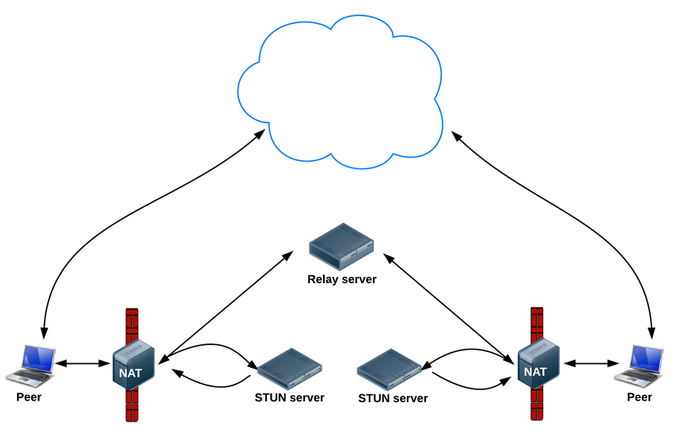
\includegraphics[height=0.30\textheight,natwidth=610,natheight=642]{figs/webrtc_network_finCandidate.png}
  	\caption{\gls{webrtc} Network: Finding connection candidates\cite{html5rock:webrtc}}
  	\label{fig:webrtc_network_finCandidate}
\end{figure} 

\begin{figure}
	\centering
    	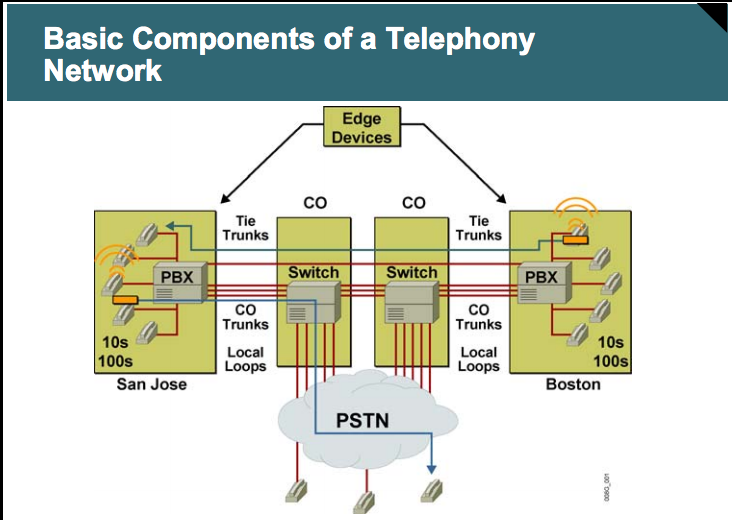
\includegraphics[height=0.40\textheight,natwidth=610,natheight=642]{figs/telephony_network.png}
  	\caption{Traditional Telephony Network}
  	\label{fig:telephony_network}
\end{figure}

\par Initially, \gls{ice} tries to connect peers directly, with the lowest possible latency, via \gls{udp}. In this process, \gls{stun} servers have a single task which is to enable a peer behind a \gls{nat} to find out its public address and port. If \gls{udp} fails, \gls{ice} tries \gls{tcp} (first \gls{http}, then \gls{https}). If direct connection fails in particular, because of enterprise \gls{nat} traversal and firewalls \gls{ice} uses an intermediary (relay) \gls{turn} server. In other words, \gls{ice} will first use \gls{stun} with \gls{udp} to directly connect peers and, if that fails, will fall back to a \gls{turn} relay server. The expression 'finding candidates' refers to the process of finding network interfaces and ports.\cite{html5rock:webrtc}

\par The difference and usage of \gls{stun} server and \gls{turn} server will be discussed more detail in Chapter \ref{chp:sys_deploy}.

\par \gls{webrtc} needs server to help users discover each other and exchange 'real world' details such as names. Then \gls{webrtc} client applications (peers) exchange network information. After that, peers exchange data information about media such as video format and resolution. Finally, \gls{webrtc} client applications can traverse \gls{nat} gateways and firewalls.

\par Compare to the traditional telephony network which is shown in Figure\ref{fig:telephony_network}\cite{web:teleVSvoip}, the main difference between these two communication network is that \gls{webrtc} is \gls{p2p} communication in \gls{stun} server scenario, after the signaling between end-peers, the media data are exchanged directly between two peers. However, in the traditional telephony, all the media data are transferred to \gls{pbx} and switches regarding to \gls{pstn}\footnote{The PSTN consists of telephone lines, fiber optic cables, microwave transmission links, cellular networks, communications satellites, and undersea telephone cables, all interconnected by switching centers, thus allowing any telephone in the world to communicate with any other. Originally a network of fixed-line analog telephone systems, the PSTN is now almost entirely digital in its core network and includes mobile and other networks, as well as fixed telephones.\cite{wiki:pstn}} then reach the other side of the peer. Even in \gls{turn} server scenario for \gls{webrtc}, the media stream is only relaying to the \gls{turn} then directly transfer to another peer, no switches involved.

\subsection{WebRTC Implementation Steps}

\begin{figure}
	\centering
    	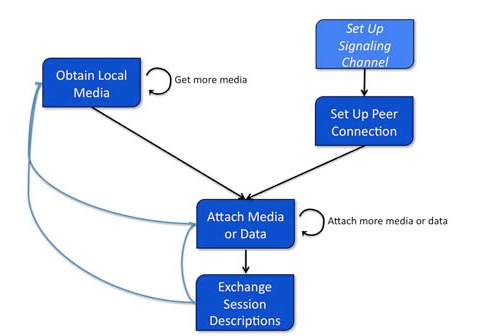
\includegraphics[width=0.80\textwidth,natwidth=610,natheight=642]{figs/webrtcApis.png}
  	\caption{WebRTC \gls{api} View with Signaling\cite{inbook:rtc-apis}}
  	\label{fig:webrtc_4steps}
\end{figure}

\noindent There are four main steps to implement a \gls{webrtc} session shown in Figure \ref{fig:webrtc_4steps}. The browser client need to obtain local media first, then set up a connection between the browser and the other peer through some signaling, after that attach the media and data channels to the connection, afterwards exchange the session description from each other. Then the media stream will automatically exchange through the real-time peer to peer media channel.

\par Each step shown in the Figure \ref{fig:webrtc_4steps} is implemented by some \gls{webrtc} \gls{api}s. More detail about how to use these \gls{webrtc} \gls{api}s to implement these steps will be covered in Chapter \ref{chp:sys_imp}. The \gls{webrtc} architecture is shown in Figure \ref{fig:webrtc_api_arch}, the main focus in this thesis will be Web \gls{api} part and transport part because Web \gls{api} is the tool to implement the \gls{webrtc} application and transport part is the key for \gls{webrtc} application to communicate with application server, media server and any other end peer in the system. 

\begin{figure}
	\centering
    	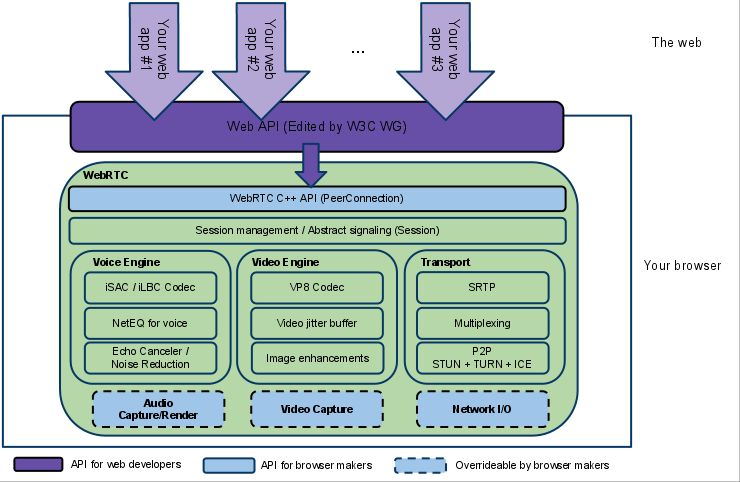
\includegraphics[width=0.80\textwidth,natwidth=610,natheight=642]{figs/WebRTCapiPic.png}
  	\caption{\gls{webrtc} architecture \cite{org:webrtc}}
  	\label{fig:webrtc_api_arch}
\end{figure}

\par Besides \gls{webrtc} \gls{api}s, signaling is the other important factor in the system. \gls{webrtc} uses \textit{RTCPeerConnection} (more about this \gls{api} will be discussed in Chapter \ref{chp:sys_imp}) to communicate streaming data between browsers, but also needs a mechanism to coordinate communication and to send control messages, a process known as signaling. Signaling methods and protocols are not specified by \gls{webrtc} by Google in purpose, then signaling is not part of the \textit{RTCPeerConnection} \gls{api} which can be decide how to implemented based on different project scenario.

\par Instead, \gls{webrtc} app developers can choose whatever messaging protocol they prefer, such as \gls{sip} or \gls{xmpp}, and any appropriate duplex (two-way) communication channel. The prototype application in this thesis will use WebSocket\footnote{WebSocket is a protocol providing full-duplex communications channels over a single TCP connection.\cite{wiki:websocket}} as signaling between \gls{webrtc} browser end point and keep use \gls{sip} as signaling for \gls{sip} end point (mobile/fixed phone based on \gls{pstn} in this case).

\noindent Signaling is used to exchange three types of information in \gls{webrtc}\cite{html5rock:webrtc}:

\begin{itemize}[topsep=-1em,parsep=0em,itemsep=0em]
 \item Session control messages: to initialize or close communication and report errors.
 \item Network configuration: to the outside world, the computer's IP address and port.
 \item Media capabilities: the codecs and resolutions can be handled by the browser and the browser it wants to communicate with.
\end{itemize}

\par The exchange of information via signaling must have completed successfully before peer-to-peer streaming can begin. For the prototype application in this thesis, the signaling has two mechanisms, one is for \gls{webrtc} browser clients and the other is for \gls{sip} clients, it will be explained in Chapter \ref{chp:sys_imp}.

\section{WebRTC Usage Cases}

\noindent After Google released the \gls{webrtc} as open source project. There are more and more web applications using it in different ways. \gls{webrtc} \gls{api}s includes three important \gls{api}s, shown below. There are mainly two types of the \gls{webrtc} applications used them in separately or cooperatively way.

\begin{itemize}[topsep=-1em,parsep=0em,itemsep=0em]
 \item \textbf{RTCPeerConnection:} audio or video calling, with facilities for encryption and bandwidth management.
  \item \textbf{MediaStream:} get access to data streams, such as from the user's camera and microphone.
 \item \textbf{RTCDataChannel:} peer-to-peer communication of generic data.
\end{itemize}

\par \textit{RTCPeerConnection} is the foundation of all \gls{webrtc} application to establish the peer to peer connection. For showing remote peer media source content and exchange the local peer media source content, the web application need to get the user's camera view and microphone sound, the \textit{MediaStream} \gls{api} is used always in real-time communication application. The following business usage cases, 'Tropo' and 'Uberconference', are in this category.

\subsection{Tropo}

\par Tropo is an application platform that enables web developers to write communication applications in the languages they already use, Groovy\footnote{Groovy is an object-oriented programming language for the Java platform. It is a dynamic language with features similar to those of Python, Ruby, Perl, and Smalltalk.\cite{wiki:groovy}}, Ruby\footnote{Ruby is a dynamic, reflective, object-oriented, general-purpose programming language. It was designed and developed in the mid-1990s by Yukihiro "Matz" Matsumoto in Japan.\cite{wiki:ruby}}, \gls{php}\footnote{PHP is a server-side scripting language designed for web development but also used as a general-purpose programming language.\cite{wiki:php}}, Python\footnote{Python is a widely used general-purpose, high-level programming language.\cite{wiki:python}} and JavaScript\footnote{JavaScript (JS) is a dynamic computer programming language.\cite{wiki:js}}, or use a Web \gls{api} which will talk with an application running on your own server through the use of \gls{http} and \gls{json}, feeding requests and processing responses back and forth as needed. Tropo is in the cloud, so it manages the headaches of dealing with infrastructure and keeping applications up and running at enterprise-grade. With Tropo, developers can build and deploy voice and telephony applications, or add voice to existing applications.\cite{web:tropo}

\par It has some advanced features, like 'Phone numbers around the world', 'Text messaging', 'Transcription', 'Call Recording', 'Conferencing', 'Text to Speech' and 'Speech Recognition'. The prototype system in this thesis will provide similar functions like 'Text messaging' and 'Conferencing'. Since Tropo is a cloud application platform, it generates its own scripts based on programming language to provide developer possibility to easily use \gls{webrtc} to communicate with other kinds of network rather than \gls{ip} network. The functions Tropo provided is implemented in application server in the prototype, the application server will handle both the \gls{sip} stack and \gls{webrtc} stack in the system. For the client, scripts will be host on the same application server for browser to access and use.

\subsection{Uberconference}

\par UberConference gives a visual interface to every conference call so callers can know who's on a call and who's speaking at any time, in addition to making many other features, such as Hangouts\footnote{Google Hangouts is an instant messaging and video chat platform developed by Google, which launched on May 15, 2013 during the keynote of its I/O development conference.\cite{wiki:hangouts}} integration and screen sharing, easy-to-use with the click of a button. It is built by the teams that brought Google Voice\footnote{Google Voice (formerly GrandCentral) is a telecommunications service by Google launched on March 11, 2009.\cite{wiki:googleVoice}} and Yahoo! Voice to tens of millions of users, UberConference launched in 2012 and is funded by Andreessen Horowitz and Google Ventures.\cite{web:uberconference}

\begin{wrapfigure}{r}{0.6\textwidth}
	\centering
    	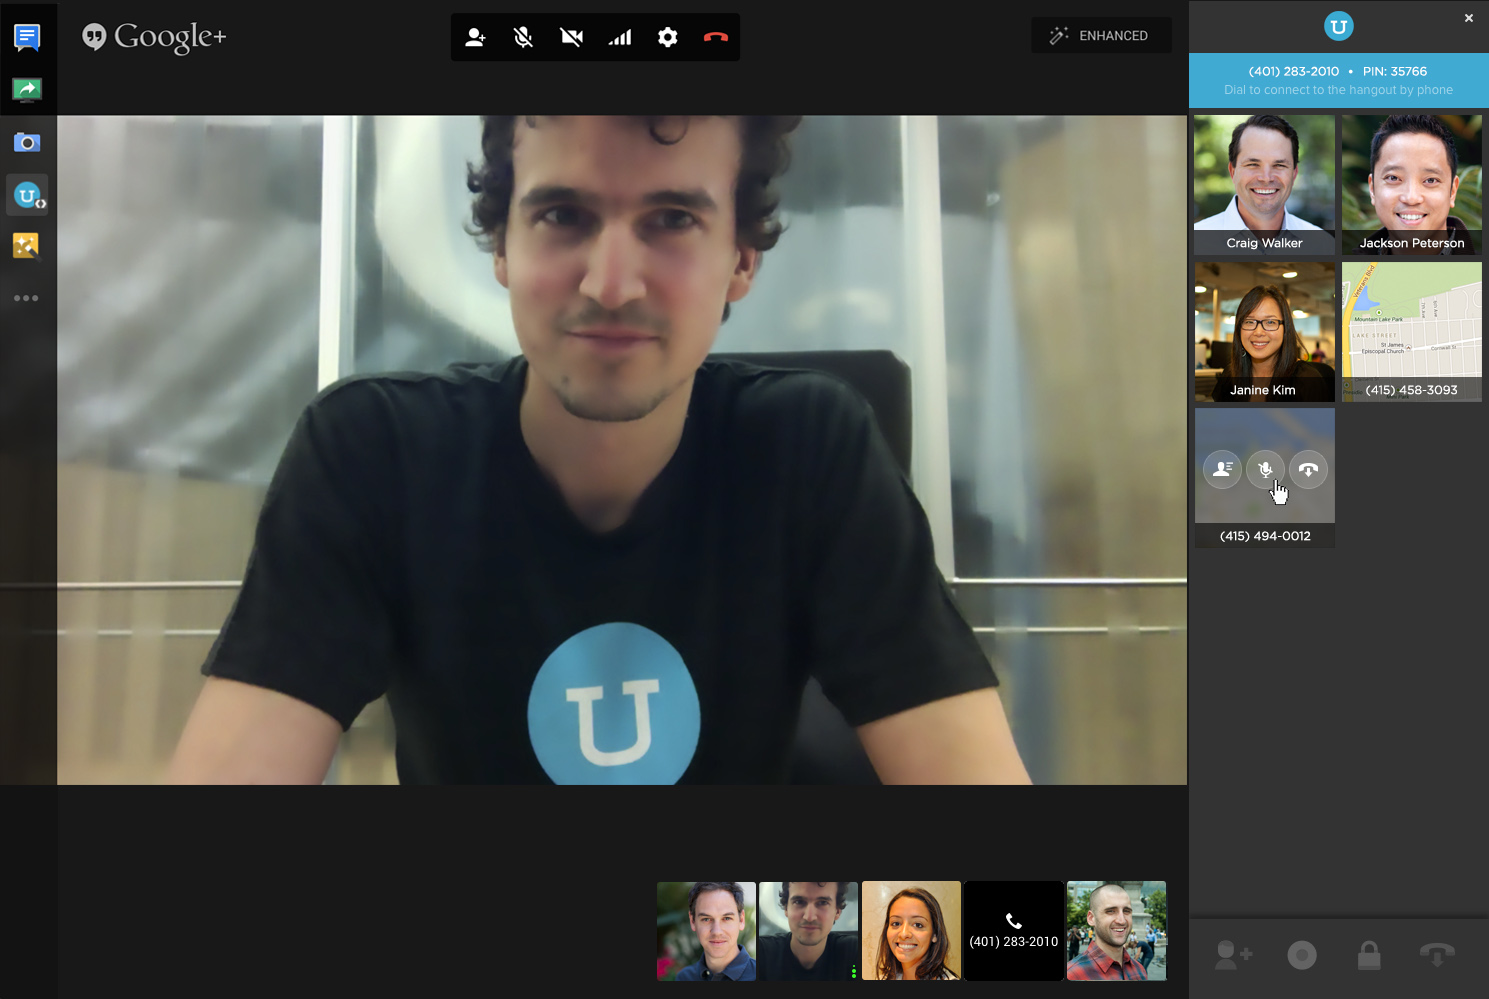
\includegraphics[width=0.58\textwidth,natwidth=610,natheight=642]{figs/uberconference_hangout.jpg}
  	\caption{UberConference integrate with Hangouts Screen shot\cite{tnw:uberconference}}
  	\label{fig:uberconference}
\end{wrapfigure}

\par The prototype system in this thesis ideally is to provide same rich media communication platform as the service provided by UberConference. In February of 2014, UberConference release the new feature which allow user to call into a Google Hangouts session with their mobile phone. The feature is shown in Figure \ref{fig:uberconference}, Once you have installed the UberConference app in Hangouts, people can join your call via phone with the help of a dedicated number. The prototype system will provide the same real-time communication service, but it allows the user to create a video conference based on \gls{webrtc} on browser by their mobile phone number and communicate with audio only mobile phone user as well. 

It will be more easier for user since they just need to remember their user credential related to their mobile phone number in order to use the prototype application rather than register another service user binding with private telephone number. And also it is more like usual telephone using because user call contacts based on their telephone number on the contact list. During the real-time conversation, the prototype application will provide user cooperation tools like instance message and file sharing in this development phase.

\subsection{Cube Slam}

\noindent Moreover, there is another important \gls{api}, \textit{RTCDataChannel} , can be used more creatively by developers to build web applications. The experiment usage cases, 'Cube Slam' and 'Webtorrent', are in this category which uses \textit{RTCDataChannel} to build \gls{p2p} data sharing without data going though the server to dispatch to other peers. It works more efficiently to handle the synchronization problem.

\par Cube Slam (shown in Figure \ref{fig:cube_slam}) is a Chrome Experiment built with \gls{webrtc} , play an old-school arcade game with your friends without downloading and installing any plug-ins. Cube Slam uses \textit{getUserMedia} to access user's webcam and microphone ,\textit{RTCPeerConnection} to stream user video to another user, and \textit{RTCDataChannel} to transfer the bits that keep the gameplay in sync. If two users are behind firewalls, \textit{RTCPeerConnection} uses a TURN  relay server (hosted on Google Compute Engine) to make the connection. However, when there are no firewalls in the way, the entire game happens directly peer-to-peer, reducing latency for players and server costs for developers.\cite{chrome:cube_slam}

\begin{figure}
	\centering
    	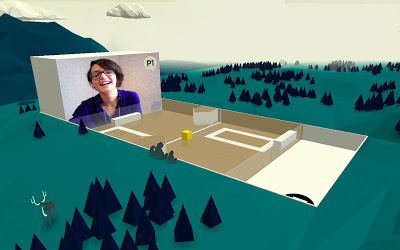
\includegraphics[width=0.8\textwidth,natwidth=610,natheight=642]{figs/cube_slam.jpg}
  	\caption{Cube Slam Game Over Screen}
  	\label{fig:cube_slam}
\end{figure}

\par The idea behind the Cube Slam is that using \textit{RTCDataChannel} to sync the player data in real-time to reduce the latency by peer to peer. \textit{RTCDataChannel} sends data securely, and supports an "unreliable" mode for cases where you want high performance but don't care about every single packet making it across the network. In the cases like games where low delay often matters more than perfect delivery, this ensures that a single stray packet doesn't slow down the whole app. The prototype application in this thesis will use WebSocket for data sharing instead of \textit{RTCDataChannel} because the media server using in this system is not support \textit{RTCDataChannel} yet, so it is not possible to create peer to peer session regarding to this issue. The \textit{RTCDataChannel} solution in prototype application will be discussed in Chapter \ref{chp:future_work}.

\subsection{Webtorrent}

\par The goal of project Webtorrent is to build a browser BitTorrent client that requires no install, no plugin, no extension, and fully-interoperates with the regular BitTorrent network. It uses \gls{webrtc} Data Channels for peer-to-peer transport. Since WebTorrent is web-first, it's simple for users who do not understand .torrent files, magnet links, NATs, etc. By making BitTorrent easier, it will be accessible to new swathes of users who were previously intimidated, confused, or unwilling to install a program on their machine to participate.\cite{github:webtorrent}

\par Since \gls{webrtc} is usually used for peer to peer communication, the \textit{RTCDataChannel} can be used in more creative way like Webtorrent. Although it need to keep the browser up and running on both ends and there will be no asynchronous nature into it, it does reduce the bandwidth required and it adds privacy as to who has access to the file being shared. Since the application can reach direct between browsers, it can use the data channel to create a low latency network, where data is shared directly without going through servers on the way. It is lower cost for the developer and more secure for the clients. For example, doing the same using a drastically larger number of web browser nodes as \gls{tor}\footnote{Tor (previously an acronym for The Onion Router) is free software for enabling online anonymity and censorship resistance. \gls{tor} directs Internet traffic through a free, worldwide, volunteer network consisting of more than five thousand relays to conceal a user's location or usage from anyone conducting network surveillance or traffic analysis.\cite{wiki:tor}}, increases the chance of privacy.This can reduce the need for “real” web servers to run services, and use those only as points of access into the dynamic network that is created ad-hoc.

\par This \textit{RTCDataChannel} usage is reasonable solution to the prototype system as well. However, the main focus of the prototype system is to integrate the \gls{webrtc} multimedia type with the \gls{voip} network against with traditional telephony network. It will not implement \textit{RTCDataChannel} function in the system, but this topic will be discussed in chapter \ref{chp:future_work}.

\section{SIP}
\noindent The prototype application in this thesis will be integrated with \gls{pstn} through \gls{sip} server. Therefore the application server implemented in this system will use \gls{sip} as signaling to communicate with \gls{sip} server to handle the signaling configuration with mobile/fixed phone end-point.

\subsection{What is SIP ?}
\noindent The \gls{sip} is a signaling communication protocol, widely used for controlling multimedia communication sessions such as voice and video calls over \gls{ip} networks.

\par The protocol defines the messages that are sent between endpoints which govern establishment, termination and other essential elements of a call. \gls{sip} can be used for creating, modifying and terminating sessions consisting of one or several media streams. \gls{sip} can be used for two-party (unicast) or multiparty (multicast) sessions. Other \gls{sip} applications include video conferencing, streaming multimedia distribution, instant messaging, presence information, file transfer, fax over \gls{ip} and online games.\cite{wiki:sip}

\par \gls{sip} works in conjunction with several other application layer protocols that identify and carry the session media. Media identification and negotiation is achieved with the \gls{sdp}. It is different key filed format than the \gls{webrtc} \gls{sdp}. For the transmission of media streams (voice, video) \gls{sdp} typically employs the \gls{rtp} or \gls{srtp}. For secure transmissions of \gls{sip} messages, the protocol can be encrypted with \gls{tls}.

\subsection{SIP Network Elements}
\noindent In normal \gls{sip} network, \gls{sip} defines user-agents as well as several types of server network elements. Two \gls{sip} endpoints can communicate without any intervening \gls{sip} infrastructure. However, this approach is often impractical for a public service, which needs directory services to locate available nodes on the network. In the system implemented of this thesis, the application server will play the roles as 'User Agent', 'Registrar' and 'Gateway' elements in the \gls{sip} network.

\noindent \textbf{User Agent}\cite{wiki:sip}:
\par A \gls{sip} \gls{ua} is a logical network end-point used to create or receive \gls{sip} messages and thereby manage a \gls{sip} session. A \gls{sip} \gls{ua} can perform the role of a \gls{uac}, which sends \gls{sip} requests, and the \gls{uas}, which receives the requests and returns a \gls{sip} response. These roles of \gls{uac} and \gls{uas} only last for the duration of a \gls{sip} transaction.

\noindent \textbf{Registrar}\cite{wiki:sip}:
\par A registrar is a \gls{sip} endpoint that accepts REGISTER requests and places the information it receives in those requests into a location service for the domain it handles. The location service links one or more \gls{ip} addresses to the \gls{sip} \gls{uri} of the registering agent. The \gls{uri} uses the sip: scheme, although other protocol schemes are possible, such as tel:. More than one user agent can register at the same \gls{uri}, with the result that all registered user agents receive the calls to the \gls{uri}.

\noindent \textbf{Gateway}\cite{wiki:sip}:
\par Gateways can be used to interface a \gls{sip} network to other networks, such as the \gls{pstn}, which use different protocols or technologies. In the prototype application, the application server is the gateway to interface a \gls{webrtc} WebSocket network. The working process will be covered in Chapter \ref{chp:sys_imp}.

\subsection{SIP messages}
\noindent Since the application server in this system will be used as \gls{sip} \gls{ua} and \gls{sip} Gateway, it will send \gls{sip} message requests to \gls{sip} server and receive \gls{sip} message requests from the \gls{sip} server.

\par One of the wonderful things about \gls{sip} is that it is a text-based protocol modeled on the request/response model used in \gls{http}. This makes it easy to debug because the messages are easy to construct and easy to see.  Contrasted with H.323\footnote{H.323 is a recommendation from the ITU Telecommunication Standardization Sector (ITU-T) that defines the protocols to provide audio-visual communication sessions on any packet network. The H.323 standard addresses call signaling and control, multimedia transport and control, and bandwidth control for point-to-point and multi-point conferences.\cite{wiki:h323}}, SIP is an exceedingly simple protocol.  Nevertheless, it has enough powerful features to model the behavior of a very complex traditional telephone \gls{pbx}.\cite{networkworld:sip}

\par There are two different types of \gls{sip} messages: requests and responses. The first line of a request has a method, defining the nature of the request, and a Request-\gls{uri}, indicating where the request should be sent.The first line of a response has a response code.

\noindent For sip requests, regarding to RFC 3261\cite{rfc:3261}, the application server in the system will use following \gls{sip} messages:

\begin{itemize}[topsep=-1em,parsep=0em,itemsep=0em]
 \item \textbf{REGISTER:} Used by a \gls{ua} to indicate its current \gls{ip} address and the \gls{url}s for which it would like to receive calls.
 \item \textbf{INVITE:} Used to establish a media session between user agents.
 \item \textbf{ACK:} Confirms reliable message exchanges.
 \item \textbf{CANCEL:} Terminates a pending request.
 \item \textbf{BYE:} Terminates a session between two users in a conference.
\end{itemize}

\noindent The \gls{sip} response types defined in RFC 3261 will be listened by application server in the following response codes\cite{wiki:sip_response_codes}:

\begin{itemize}[topsep=-1em,parsep=0em,itemsep=0em]
 \item \textbf{100 Trying:} Extended search being performed may take a significant time so a forking proxy must send a 100 Trying response.
 \item \textbf{180 Ringing:} Destination user agent received INVITE, and is alerting user of call.
 \item \textbf{200 OK:} Indicates the request was successful.
 \item \textbf{400 Bad Request:} The request could not be understood due to malformed syntax.
 \item \textbf{401 Unauthorized:} The request requires user authentication. This response is issued by \gls{uas}s and registrars.
 \item \textbf{408 Request Timeout:} Couldn't find the user in time. The server could not produce a response within a suitable amount of time, for example, if it could not determine the location of the user in time. The client MAY repeat the request without modifications at any later time.
 \item \textbf{480 Temporarily Unavailable:} Callee currently unavailable.
 \item \textbf{486 Busy Here:} Callee is busy.
\end{itemize}

\par By listening these \gls{sip} response, the application will send requests to either \gls{webrtc} browser client or \gls{sip} client to play as the gateway role in the system. This gateway mechanism will be introduced in Chapter \ref{chp:sys_design}.

\section{Prototype System Working Flow}

\noindent To connect with the traditional telephony network, the \gls{voip} system bridges the \gls{pstn} and the \gls{ip} network. \gls{voip} systems employ session control and signaling protocols to control the signaling, set-up, and tear-down of calls. They transport audio streams over \gls{ip} networks using special media delivery protocols that encode voice, audio, video with audio codecs, and video codecs as Digital audio by streaming media. In the prototype system, \gls{sip} signaling is used because of its widely usage and current target \gls{pstn} has \gls{sip} server support.

\begin{figure}
	\centering
    	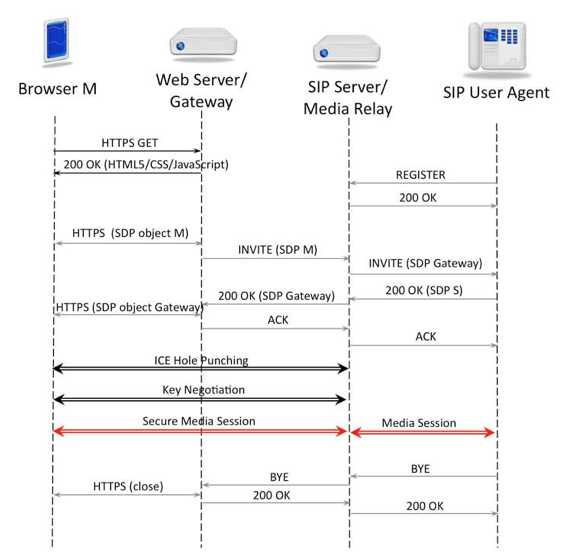
\includegraphics[width=0.60\textheight,natwidth=610,natheight=642]{figs/system_work_flow.png}
  	\caption{Prototype System Working Diagram \cite{inbook:sys_work_diagram}}
  	\label{fig:sys_work_diagram}
\end{figure}

\par The Figure \ref{fig:sys_work_diagram} shows the basic working flow of the prototype system. The Web Server/ Gateway is the application server in the prototyep system, it mainly bridges the \gls{webrtc} browser client with other \gls{webrtc} clients and the \gls{sip} network. The \gls{sip} server bridges the \gls{sip} network and \gls{pstn} network or traditional telephony network. And also the Media Relay server relay all the media stream from different end clients. In the prototype system, there is another media server besides the media relay function provided by \gls{sip} server because the media server needs to handle different media \gls{sdp} in signalings which are \gls{webrtc} \gls{sdp} and \gls{sip} \gls{sdp}. The media server used in the prototype system is provided by Dialogic, the Network Fuel company, which is called PowerMedia XMS v2.1\footnote{PowerMedia XMS is pre-integrated with a variety of application servers and signaling gateways with HTTP-to-SIP (H2S) functionality and rapidly integrates with others using its web API or standard interfaces.}. PowerMedia XMS acts as a WebRTC Media Gateway to mediate WebRTC media-plane differences from those of typical existing VoIP networks including encryption interworking, transcoding, and client-based NAT traversal support. The reason to use this media server is to avoid hard-code transition between \gls{webrtc} \gls{sdp} and \gls{sip} \gls{sdp}. Then the end client no matter is a \gls{webrtc} client or a \gls{sip} client, they will communicate with the same signaling client in their aspect.

\par Moreover, since the media server is used in this case, during the multiple end-point conversation, each end-point will only exchange their media stream to the single end-point on the media server (PowerMedia XMS server), it will make light client and centralized media server control. The benefit of this system architecture will be discussed more in the Chapter \ref{chp:sys_design}.

\par Therefore, in the Figure \ref{fig:sys_work_diagram}, all the end point keep using their own original signaling protocol to communicate with different servers of the prototype system in order to reach different scope end point.

\section{Prototype Working Scenario}

\noindent The prototype system in this thesis will pay more attention on the real-time communication usage of \gls{webrtc}. The main purpose of the system is to combine internet browser user and traditional telephony user without complicate instillation, plugin and extension. There are two typical working scenarios of the prototype system will be described below.

\subsection{Advanced 'one-number' communication platform}

\par Adam is a typical Facebook\footnote{Facebook is an online social networking service.} user and he does synchronize his contact list through Google Contacts\footnote{Google Contacts is Google's contact management tool that is available in its free email service Gmail, as a standalone service, and as a part of Google's business-oriented suite of web apps Google Apps.\cite{wiki:google_contacts}} by his smart phone. Now his operator provides user credential from his telephone number to him. Then Adam just login on his operator 'FellowPhone' web page, now he can import his contacts list through his Google contact list. After that, he can see if his contact person is online by using the same web application 'FellowPhone' or not. He can also import his Facebook friends list and fulfill the friends list with his contacts list information. Therefore, Adam can see if his facebook friends online or not. If his facebook friends/ Google contacts are online and use 'FellowPhone' web application from their operator, Adam can invite them have a video conference otherwise his friends are not online then he can still invite them into the video conference but through his friends mobile phone with only audio sound.

\par During the video conference, Adam can send his online friends files and instance messages (website links, video links and so on). Moreover, his offline friends in the same conference will get the same information as text \gls{sms}. Adam can reach his friends wherever they are and no matter if they are online or not as long as they have their mobile phone. 

\subsection{Multiple doctors consultation room}

\par Eve is a 70-year-old lady, she lives with her children in their house. But at the day time, her children go to work, she need take care of herself. She has appointment with her doctor about her backache. But she can not go to hospital or family doctor office by her own. Then she uses her mobile phone to call her family doctor. Her family doctor, Isak, uses the prototype service from his company and operator. When Eve call to her doctor for help, Isak answered her phone and tried to get her previous medical information from his working system. Then he found out that Eve had other doctor about her back treatment before. He can just login in the prototype system and find out if the other doctor is at work (online in the system). Eve's previous doctor, Stella, she has the treatment log about Eve. She got invitation to join the current conversion with Isak and Eve. She can send message to Isak and share the treatment log with Isak if it is necessary. She can also listen to the talk between Isak and Eve about the new update of the treatment to give suggestion. Isak can ask for more different doctors in the system for advice and consultation to help for Eve case.

\par In Eve aspect, she only calls doctor Isak, but she can got help from more than one doctor at the same time. If it is necessary, she can use the computer to login the same system to have video conference with different doctors for her case. The only thing required for her is a telephone number and a mobile phone.